%%%   Local Variables:
%%%   mode: latex
%%%   TeX-master: "IS1apuntes"
%%%   End:


\section{Introducción}

Podemos encontrar dos paradigmas principales para la construcción de sistemas
software. Por un lado, tenemos el \textbf{Estructurado} y por otro el
\textbf{Orientado a Objetos}. Asimismo, el Diseño Estructurado se basa en tres
fundamentos:

\begin{itemize}[noitemsep]
\item \emph{Top-Down}
\item Sistemas como funciones.
\item Datos y funciones separados.
\end{itemize}


\section{Análisis vs Diseño}

Los lenguajes de alto nivel en el pasado son los lenguajes de bajo nivel del futuro\footnote{Pues eso, funcional.}, así mismo las técnicas de \textbf{análisis} de ayer son técnicas de \textbf{diseño} de hoy.

Los problemas reales de los usuarios son problemas de organización, monitorización, control, etc; Por tanto los problemas no son ni \textit{estructurados} ni \textit{orientados a objetos}, pero las \textbf{soluciones} sí.

El análisis pretende comprender algo que \textbf{ya existe}: estudiarlo, delimitarlo, clasificarlo...

Son tareas del análisis, por ejemplo:

\begin{itemize}[noitemsep]
\item Realizar un estudio del mercado entes del lanzamiento de un producto.
\item Encontrar las causas del fracaso de un proyecto software.
\item Estudiar las características del terreno donde se construirá un edificio.
\end{itemize}

En general se encarga de comprender un problema antes de resolverlo \textbf{(requisitos)}.

El diseño busca crear \textbf{algo que no existe}: elaborar un plan antes de comenzar a construir.

Ejemplos de tareas de diseño son:

\begin{itemize}[noitemsep]
\item \textbf{Crear} un producto para lanzarlo al mercado.
\item \textbf{Elaborar} los planos de un edificio.
\end{itemize}

En general el diseño se encarga de utilizar cierta tecnología para resolver un problema \textbf{(DFDs, OO)}.

En Ingeniería de Software se denominaba \textit{\textbf{``Análisis''}} de problemas a lo que, en realidad, era un \textit{\textbf{``Diseño''}} de soluciones.\index{análisis}

\subsection{Enfoque de Yourdon}
\textit{Nota: A pesar de que el libro de Yourdon se denomina ``Análisis Estructurado Moderno'' lo consideraremos como si fuera diseño. Su técnica no sirve para describir problemas, sino soluciones (tecnologías).}

\begin{itemize}[noitemsep]
\item Se basa en una serie de notaciones bastante conocidas cómo \textbf{DFDs}, \textbf{E/R}, etc.
\item Se mantiene una relación entre las notaciones.
\item Su objetivo es elaborar un \textbf{``Modelo esencial''} del sistema.
\item No es top-down, sino \textbf{middle-up}, \textbf{middle-down}.
\item La construcción del Diagrama de Flujo de Datos está \textbf{dirigida por acontecimientos}.
\item Pese a ser moderno, es \textbf{antiguo}, pero no tanto como el enfoque puramente \textit{top-down}.
\end{itemize}

\section{Notaciones}
Las notaciones que describiremos son:

\begin{itemize}[noitemsep]
\item Diagrama de Fujo de Datos (DFDs).
\item Diccionario de Datos (DDs).
\item Especificación de procesos.
\item Entidad/Relación (E/R).
\end{itemize}

\subsection{Diagramas de Flujo de Datos} %% TODO
La \textbf{notación} se escribe a continuación:

\begin{center}
  \centering
  \begin{tabular}[h]{ l r }
    Procesos                            & 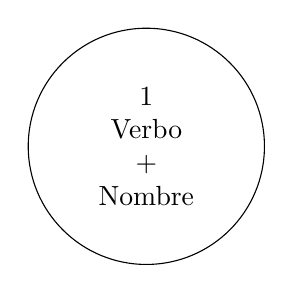
\begin{tikzpicture} \draw circle [radius=1.5] node[text width=2cm, text centered] {1\\ Verbo\\ +\\ Nombre}; \end{tikzpicture} \\
    & \\
    Flujos                              & 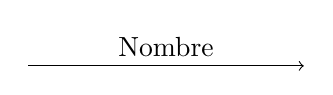
\begin{tikzpicture} \draw [->]  (0,0) -- node [midway, above] {Nombre} (3.5,0); \end{tikzpicture} \\
    & \\
    Almacenes                           & 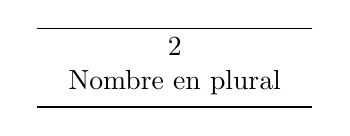
\begin{tikzpicture} \path[shape=coordinate] (0,0) coordinate(dl) (3.5,0) coordinate(dr)
                                                                                      (3.5,1) coordinate(ul) (0,1) coordinate(ur);
                                                                                      \filldraw[thin] (dl) -- (dr) (ul) -- (ur)
                                                                                      node[midway, below, text width=3.5cm, text centered] {2\\ Nombre en plural};
                                          \end{tikzpicture} \\
    & \\
    Terminadores (Entidades Externas)   & 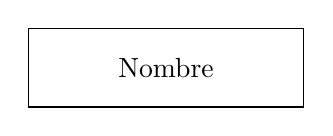
\begin{tikzpicture} \draw rectangle (3.5,1) node[pos=.5] {Nombre}; \end{tikzpicture} \\
  \end{tabular}
\end{center}

Las \textbf{reglas} son:

\begin{itemize}[noitemsep]
\item Nombres con significado.
\item Numerar los procesos NO implica secuencia.
\item Evitar DFDs complejos.
\item Todo DFD se redibuja varias veces.
\end{itemize}

La \textbf{regla del balanceo} mantiene la consistencia entre las entradas y salidas de una burbuja padre y las entradas y salidas de todas sus burbujas hijas.

Para preservar la \textbf{consistencia lógica} de un Diagrama de Flujo de Datos hay que \textbf{evitar}:

\begin{itemize}[noitemsep]
\item Sumideros infinitos.
\item Generaciones espontáneas.
\item Flujos y procesos no etiquetados.
\item Cuidado con los almacenes de sólo lectura o sólo escritura.
\end{itemize}


\subsection{Diccionario de Datos} %% TODO
Un Diccionario de Datos es una \textbf{lista organizada} de todos los datos, que describe el \textbf{significado} y la \textbf{composición} de los flujos y almacenes, así como también las \textbf{relaciones} entre almacenes mediante un E/R.

Su \textbf{notación} es:

\begin{center}
  \begin{tabular}[h]{ l | l }
    \textbf{Símbolo}   & \textbf{Significado} \\
    \hline
    =                  & \textit{se define como} \\
    +                  & \textit{y} \\
    ()                 & opcional \\
    \{\}               & iteración \\
    \big[\big]         & separa alternativas \\
    *...*              & define datos elementales \\
    **                 & comentario \\
    @                  & identificador (clave) \\
    |                  & alternativa \\
  \end{tabular}
\end{center}

\subsection{Especificaciones de proceso}

Son sólo para los procesos (burbujas) de más bajo nivel. Se puede utilizar:

\begin{itemize}[noitemsep]
\item Lenguaje estructurado.
\item Pre/post.
\item Tablas de decisión.
\item Gráficas.
\item Lenguaje natural.
\item Flow-charts.
\end{itemize}

\textbf{Presentación por niveles}:

\begin{itemize}[noitemsep]
\item Los DFDs se presentan TOP-DOWN. Esto NO quiere decir que se construyan TOP-DOWN.
\item El orden de presentación es: Diagrama de Contexto, Diagrama 0, Diagrama 1, etc.
\item ¿Hasta donde?: Se detiene la descomposición cuando las burbujas pueden especificarse como procesos sencillos (en menos de una página).
\item Sistemas sencillos: 2-3 niveles en total; medianos: 3-6; grandes: 5-8.
\end{itemize}


\subsection{Entidad/Relación}

Las \textbf{entidades}:

\begin{itemize}[noitemsep]
\item Representan conjuntos de individuos.
\item Cada individuo puede identificarse de manera única.
\item Cada uno juega un papel necesario en el sistema.
\end{itemize}

Yourdon no utiliza atributos en el diagrama pero sí en el Diccionario de Datos.

Las \textbf{relaciones} representan conjuntos de conexiones con sus cardinalidades.

Las \textbf{entidades asociativas} pueden verse como \textit{entidades que contienen los atributos de una relación}. Se utilizan para representar relaciones acerca de las cuales se quiere guardar alguna información. Como por ejemplo:

\textit{Un cliente compra artículos y queremos guardar información acerca del día y hora de la compra.}

En este caso ``Día'' y ``Hora'' serían \textbf{propiedades} de la relación, pero no de ``Cliente'' ni de ``Artículo''.

En el Diccionario de Datos tendríamos:

\begin{itemize}[noitemsep]
\item Cliente = @DNI + Nombre + Dirección + Telf.
\item Artículo = @Código + Descripción + Precio.
\item Compra = @DNI + @Código + Día + Hora.
\end{itemize}

A continuación se muestra un ejemplo de E/R con dos entidades
(Persona y Herramienta) y una relación (Usa):

\begin{center}
  \begin{tikzpicture}[node  distance =7em]
    \node[entity] (persona) {Persona};
    \node[relationship] (usa) [right  of=persona] {Usa} edge (persona);
    \node[entity] (herramienta) [right  of=usa] {Hrramienta} edge (usa);
  \end{tikzpicture}
\end{center}

Las reglas para la construcción de un modelo E/R son las siguientes:

\begin{itemize}[noitemsep]
\item Entrevistas, documentos: permiten la \textbf{identificación} de entidades.
\item Se refinan y desarrollan en paralelo a los DFDs y DDs para mantener consistencia.
\item Simplificar:

  Eliminar objetos de instancia única.

  Eliminar relaciones derivadas (calculables).

\item Regla heurística: si no somos capaces de imaginar al menos 3 registros de una entidad, malo.
\end{itemize}

\section{Relación entre notaciones}

\textbf{1. Diagrama de Flujo de Datos y Diccionario de Datos}

\begin{itemize}[noitemsep]
\item Todo flujo y almacén del DFD deben definirse en el DD y viceversa.
\end{itemize}

\textbf{2. Diagrama de Flujo de Datos y Especificación de Proceso}

\begin{itemize}[noitemsep]
\item Toda burbuja del DFD debe asociarse con una burbuja del nivel inferior, o con una especificación de proceso pero \textbf{no ambos}.
\item Toda especificación de proceso debe asociarse a una burbuja de bajo nivel.
\item Las entradas y salidas deben coincidir.
\end{itemize}

\textbf{3. Especificación de Proceso con Diagrama de Flujo de Datos y Diccionario de Datos}

\begin{itemize}[noitemsep]
\item Los datos referenciados en la Especificación de Proceso deben coincidir con nombres de flujos o almacenes conectados a la burbuja, ser término local (variable local) o ser un componente del flujo o almacén.
\end{itemize}

\textbf{4. Diccionario de Datos con Diagrama de Flujo de Datos y Especificación de Proceso.}

\begin{itemize}[noitemsep]
\item Toda entrada del DD debe tener referencia en una Esp. Proc, un DFD o en el propio DD.
\end{itemize}

\textbf{5. Entidad/Relación con Diagrama de Flujo de Datos y Especificación de Proceso.}

\begin{itemize}[noitemsep]
\item Todo almacén del DFD debe corresponder a una entidad o entidad asociativa.
\item Toda entidad, relación o entidad asociativa del E/R debe reflejarse en algún almacén del DFD.
\item Los nombres deben coincidir: plural en DFD, singular en ER. Deben definirse ambas en el DD (ver a continuación).
\item Las instancias de las entidades y las relaciones del ER deben ser creadas o eliminadas por algún proceso.
\item Alguna burbuja del DFD define valores para cada componente de datos.
\item Alguna burbuja del DFD usa los valores de cada componente de datos.
\end{itemize}

\textbf{6. Entidad/Relación: extensiones al Diccionario de Datos.}

\begin{itemize}[noitemsep]
\item En general, las entidades se nombran en singular y los almacenes en plural.
\item Los atributos de las entidades se pueden especificar en el DD.
\end{itemize}

\section{Proceso de Construcción}

Consiste en elaborar los dos componentes del llamado \textit{Modelo Esencial}. Para lo que se construirá:

\subsection{Construcción del Modelo Ambiental}

\begin{itemize}[noitemsep]
\item Escribir en un párrafo el \textbf{propósito del sistema}.
\item Construir el \textbf{diagrama de contexto} (preliminar identificando las entidades externas).
\item Construir una \textbf{lista de acontecimientos}.
\end{itemize}

Una \textit{lista de acontecimientos} es una lista narrativa de los estímulos que ocurren en el mundo exterior a los cuales el sistema debe responder. Los hay de tres tipos:

\begin{itemize}[noitemsep]
\item \textbf{Flujo}: se asocian con la llegada de algún flujo.
\item \textbf{Temporal}: se disparan a una determinada hora.
\item \textbf{Control}: (no los tratamos).
\end{itemize}

\textit{Nota: los flujos y los acontecimientos son cosas distintas. No hay corrrespondencia uno-uno entre ambos.}

Los acontecimientos deben de contemplarse de fuera del sistema hacia dentro. Por ejemplo:

\textbf{Mal}: \textit{El sistema recibe el pedido del cliente}.

\textbf{Bien}: \textit{El cliente hace un pedido}.

La construcción de la \textit{lista de acontecimientos} se realiza \textbf{a partir} de las \textit{entidades externas}, pero el \textit{Diagrama de Contexto} se puede hacer \textbf{a la vez} que la \textit{Lista de acontecimientos}, se refinan mutuamente.

Los flujos del Diagrama de Contexto son el medio utilizado para la comunicación sistema-entorno. Los \textbf{flujos de entrada} son \textbf{utilizados} por los \textit{acontecimientos} y los \textbf{flujos de salida} son \textbf{respuestas} a los \textit{acontecimientos}.

\begin{itemize}[noitemsep]
\item Todo \textbf{acontecimiento no temporal} debe tener \textbf{entradas} para que el sistema pueda detectarlo.
\item Todo acontecimiento debe producir una \textbf{salida} inmediata y/o un \textbf{almacenamiento} de datos.
\end{itemize}


\subsection{Construcción de un Modelo de Comportamiento preliminar} %% TODO ejemplos

Consiste en desarrollar un \textit{Daigrama de Flujo de Datos} y un diagrama \textit{E/R} \textbf{preliminares}, además de las entradas iniciales del \textit{Diccionario de Datos}. Se opone al enfoque clásico debido a que \textbf{no es} top-down.

\begin{itemize}[noitemsep]
\item Se \textbf{dibuja} una burbuja o proceso por cada acontecimiento de la lista. El nombre de la burbuja describe la respuesta que se debe dar al acontecimiento.
\item Se \textbf{dibujan} las entradas, salidas y almacenes apropiados (conectados a la burbuja).
\item Se \textbf{conectan} las burbujas (de los acontecimientos) mediante almacenes.
\item En \textbf{paralelo} se contruye el diagrama \textit{E/R}.
\end{itemize}


\subsection{Acabado del Modelo}

\begin{itemize}[noitemsep]
\item Para finalizar el modelo se debe realizar una \textbf{Nivelación ascendente} hasta llegar al Diagrama de Contexto.

  - Los procesos o burbujas se agrupan por respuestas relacionadas.

  - Según se asciende se ocultan los almacenes internos a una agrupación de procesos. \textit{Sugerencia: hacer agregados de 7 +- 2 burbujas}.

\item Puede requerirse nivelación ascendente.
\item Completar el Diccionario de Datos.
\item Completar la especificación del proceso (al final).
\item En \textbf{paralelo} acabar el diagrama E/R.
\end{itemize}
